\documentclass[a4paper,11pt]{article}

\pdfoutput=1
%\usepackage{jcappub}
\usepackage{txfonts}
\usepackage{threeparttable}
%\usepackage{aas_macros}
\usepackage{graphicx}
\usepackage{subfigure}
\usepackage{url}
\usepackage{amsmath}

\begin{document}

Dear Prof. Asantha Cooray,
\\

Thank you very much for forwarding the referee report to us. Again, we are grateful to the referee for the helpful suggestions.
\\

We have revised our manuscript carefully in terms of the referee report, with new revisions marked in boldface. We sincerely hope that this newly revised version is qualified to be accepted for publication in your journal.
\\

For the reply to the referee report, please see below.
\\

Best wishes,
\\

Xiao-Lei Meng
\\
\\

Responses to the referee report is as follows,
\\

Firstly, we thank the anonymous referee again for providing helpful suggestions. We have revised our manuscript cautiously in terms of the referee report, with new revisions marked in boldface. Below, we give a detailed description of our revisions.
\\
\\
COMMENT:
\\
(1) First of all, the definition of $\gamma'$ is unclear. Abstract and Introduction say $\rho_{tot} \propto r^{-\gamma'}$ and an isothermal profile corresponds to $\gamma'$ = 2. However this is inconsistent with Eq. (4.3) in which $\gamma'$ = 1 reduces to an isothermal case. This is important because the  interpretation of $\gamma_{out}/\gamma_{in}$ shown e.g., Fig. 7 is different between $\gamma'$ = 2 and $\gamma'$ = 1 (as $\bigtriangleup \gamma'$ = 0.02 translates into $\bigtriangleup (\gamma'_{out}/\gamma'_{in})$ = 0.01 and 0.02, respectively).
\\

RESPONSE:
\\


----------------------------------------------------------------------
\\
COMMENT:
\\
(2) It is mentioned that the Gaussian PSFs are adopted for Euclid, WFIRST, and LSST. I’m a little bit concerned about this, because PSFs are known to be more extended that Gaussian (particularly for space observations). They are better described by the Moffat profile. Is this difference of the PSF not important? In fact it looks straightforward to repeat the analysis for several different PSF shapes (different $\beta$ in the Moffat profile for example) to check this effect.
\\

RESPONSE:
\\
\begin{figure}
\begin{center}
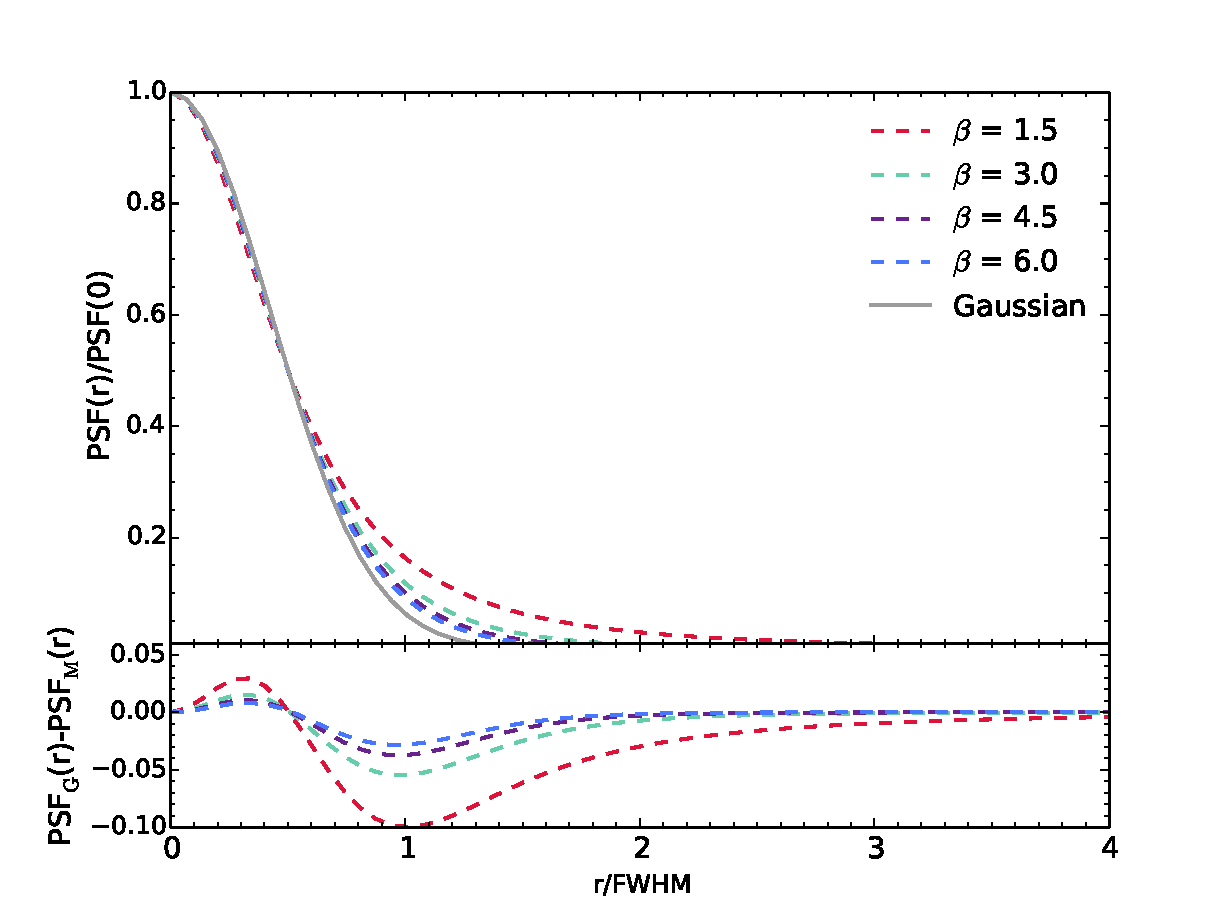
\includegraphics[width=0.9\textwidth]{psf_gaussian_moffat_correct.pdf}
\end{center}
\caption{Top panel: The normalized intensity profile of the Gaussian PSFs and Moffat PSFs with different values of $\beta$ for WFIRST. Bottom panel: The differences between these normalized Gaussian profile [PSF$_{\mathrm{G}}$(r)] and the normalized Moffat profile [PSF$_{\mathrm{M}}$(r)]. Note that the Moffat profile contains the Gaussian profile in a extraordinary case ($\beta \rightarrow \infty$).}
\label{fig:psf_g_m}
\end{figure}

\begin{table*}\footnotesize
\begin{center}
\caption{Precision on the $\gamma'$ with Gaussian and Moffat PSF for WFIRST}
\begin{tabular}{lcccccccccccccc|}
\hline \hline
Lens Name & Gaussian & Moffat & Moffat & Moffat & Moffat
\\
& & ($\beta$=1.5) & ($\beta$=3.0) & ($\beta$=4.5) & ($\beta$=6.0) \\
\hline
fainter system$^a$ & 0.021 & 0.032 & 0.028 & 0.025 & 0.023 \\
fainter system$^b$ & 0.023 & 0.036 & 0.035 & 0.033 & 0.030 \\
brighter system$^b$ & 0.0044 & 0.0065 & 0.0062 & 0.0048 & 0.0044 \\
brighter system$^a$ & 0.0016 & 0.0022 & 0.0017 & 0.0017 & 0.0015 \\
\hline
\hline
\end{tabular}
\begin{tablenotes}
\item
Precision on the mass density profile slope $\gamma'$ with Gaussian and Moffat PSFs for WFIRST. This table represents the results for fainter and brighter systems with 4 and 2 QSO images. It is shown that as $\beta$ increases the Moffat PSF tends to approximate the core of the Gaussian PSF. \\
$^a$ This configuration yields 4 QSO images. \\
$^b$ This configuration yields 2 QSO images. \\
\end{tablenotes}
\end{center}
\end{table*}

----------------------------------------------------------------------
\\
COMMENT
\\
(3) I should note that Kochanek et al. (2001) is among the first who emphasized the importance of lensed host galaxies for time delay cosmography and demonstrated how it breaks the degeneracy in lens mass models.
\\

RESPONSE:
\\ 


----------------------------------------------------------------------
\\
COMMENT:
\\
(4) Throughout the paper the authors ignore the PSF uncertainty and assume the perfect knowledge about the PSF. While I understand the authors’ point that by doing so the results represent a lower limit of the total uncertainty, I’d like to see a more extensive discussion on how the PSF uncertainty would propagate into $\gamma'$, given the critical importance of accurate PSF characterizations for AO observations. In Introduction the authors mention Marshall et al. and Lagattuta et al., but these papers are not very relevant in this context as systems studied in those papers are more like galaxy-galaxy strong lensing. In the case of quasar lensing, there must be a degeneracy between the PSF wing (from quasar images) and surface brightness profile of a lensed host galaxy, which has to be carefully addressed. Agnello et al. mentioned in the paper did not fully take account of the PSF uncertainty. In a recent paper by Rusu et al. (2015) adopted a parametrized PSF model and marginalized over PSF parameters when deriving physical parameters, and thus should be helpful in discussing potential impacts of PSF uncertainties and possible future extensions of the present paper to address the propagation of PSF uncertainties to the final result.
\\

RESPONSE:
\\ 
--------------------------------------------------------------------
\\
COMMENT:
\\
(5) In Sec. 3.1: “... of currently known lenses, selected from the Sloan Digital Sky Survey,” The current largest quasar lens sample comes from the SDSS Quasar Lens Search, containing more than 50 quasar lenses. It would be informative to give a quantitative description of the SQLS sample (typical magnitudes, quad/double ratio, etc), citing references.
\\

RESPONSE:
\\

-------------------------------------------------------------------
\\
COMMENT:
\\
(6) Also in Sec. 3.1: “As in the real-system used as inspiration” This sounds a bit odd, because SLACS and SL2S (which that sentence is referring) are not quasar lens surveys but galaxy-galaxy strong lens surveys. For example typical redshifts can be quite different.
\\

RESPONSE:
\\

------------------------------------------------------------------
\\
COMMENT:
\\
(7) Sec 3.2: “... are listed in Table 2 and Table 3.” In fact light and lens models are described later in Sec. 4, so at this point readers have no idea what these parameters mean.
\\

RESPONSE:
\\

------------------------------------------------------------------
\\
COMMENT:
\\
(8) The authors choose a quasar 1 mag brighter than the host galaxy in their simulations. It would be useful to check previous analysis of lensed quasar hosts to see how typical this assumption is compared with observed lensed quasar systems. For example Peng et al. (2006) analyzed a large sample of quasar lenses using HST. Rusu et al. (2015) mentioned above also added several more quasar lens systems with host detections.
\\

RESPONSE:
\\

-----------------------------------------------------------------
\\
COMMENT:
\\
(9) Is the quasar always placed at the center of the host galaxy? This may sound obvious, but looking at Fig. 4 lensed quasar host appears to be offseted from the quasar image. Of course this is not impossible, as a nice example was given in Agnello et al., but this kind of configuration is also not very common.
\\

RESPONSE:
\\

----------------------------------------------------------------
\\
COMMENT:
\\
(10) It looks like lensing galaxies are not shown in Figs. 3-6, I guess this is just to better show quasar images and host galaxies. If so this point should be clearly mentioned in the paper. In practice a lensing galaxy is fitted simultaneously (if I understand correctly), so it may be helpful to show simulated images with lensing galaxies as well.
\\

RESPONSE:
\\

---------------------------------------------------------------
\\
COMMENT:
\\
(11) In the non-linear fitting described in Sec. 4.2, is the sky level not included as a fitting parameter? Or the sky level is fixed to the true value during fitting?
\\

RESPONSE:
\\

---------------------------------------------------------------
\\
COMMENT:
\\
(12) In Sec. 4.3 and 5 there are sentences like “determine $\gamma'$ with 2\% precision”. This is related to my first comment, suppose that the input $\gamma'$ value is 2, “2\% precision” is different from $\gamma'$ uncertainties of 0.02. If one wants to determine H0 with 2\% accuracy, $\gamma'$ has to be deter- mined with an accuracy of 0.02, which corresponds to 1\% precision of $\gamma'$ determination for the fiducial $\gamma'$ value of 2. Please clarify.
\\

RESPONSE:
\\

---------------------------------------------------------------
\\
COMMENT:
\\
(13) In Sec. 5: “we generate 30 mock systems” These mock systems refer to different noise realizations of the same input image?
\\

RESPONSE:
\\

---------------------------------------------------------------
\\
COMMENT:
\\
(14) Figs. 7-10: I don’t quite understand the insert in each panel. If I read the caption literally, x and y axes refer to the same quantity and therefore all the points lie exactly on the $y = x$ line? Then what information does this plot carry?
\\

RESPONSE:
\\

----------------------------------------------------------------
\\
COMMENT:
\\
(15) It would be very useful to add a summary table that lists all the estimated uncertainties on $\gamma'$, as it is sort of painful to read off those values from the Figures.
\\

RESPONSE:
\\

---------------------------------------------------------






\end{document}